\documentclass[Main.tex]{subfiles} 
\begin{document}

\subsection{Sprint 3}
I Sprint 3 blev Accepttesten rettet til, s� den passede med Use Case-beskrivelserne samtidig med, at nye emner blev p�begyndt:
\\
\begin{wrapfigure}{r}{0.6\textwidth}
	\vspace{-20pt}
    \centering
	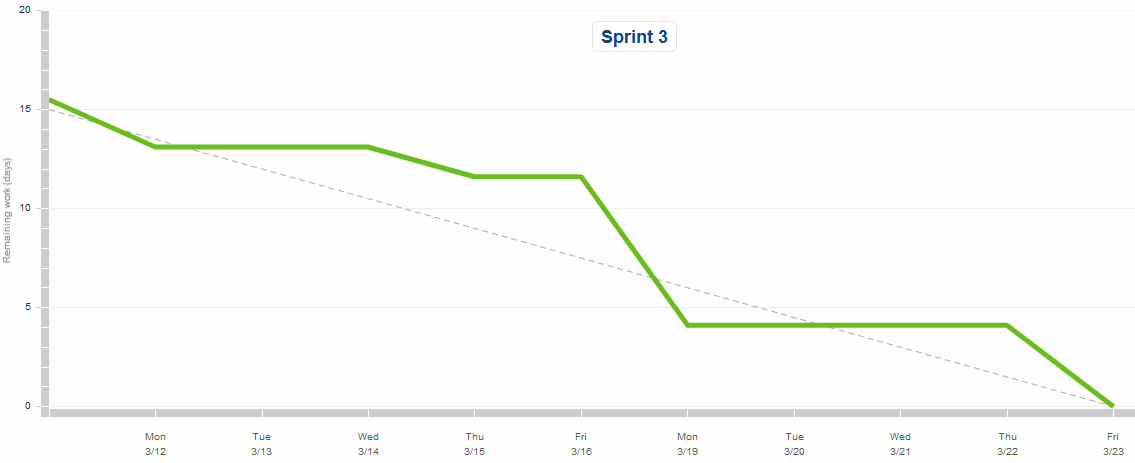
\includegraphics[scale=0.25]{Billeder/Sprint3_burn.png}
	\vspace{-20pt}
	\caption{Burndown chart for sprint 3}
  \label{fig:sprint3}
  \vspace{-10pt}
\end{wrapfigure}
Her kan n�vnes at der blev p�begyndt en IDE til at definere gruppens eget programmeringssprog. Efter at have diskuteret programmeringssproget til denne, endte valget med at falde p� \textit{Iron Python}, hvilket ogs� gav muligheden for at implementere \textit{Intellisense}.
\\
\\
V�gten der skulle bruges til at finde klodsernes densitet blev p�begyndt, og der blev lavet et udkast til, hvordan simuleringen af robotten kunne se ud.
\\
\\
Derudover blev et funktionelt program lavet, der kunne tage klodser fra transportb�ndet og flytte dem til v�gten. Alle disse ting blev fremvist for kunden i et sprint review.

\end{document}